\chapter{Experiments and Results}
\label{chap5}

In this chapter, I describe the experimental setup, provide details on the experimental procedure, and finally present and discuss environment property prediction results obtained through the prediction framework.

%FIGURE ()
\begin{figure}[]
	\centering
	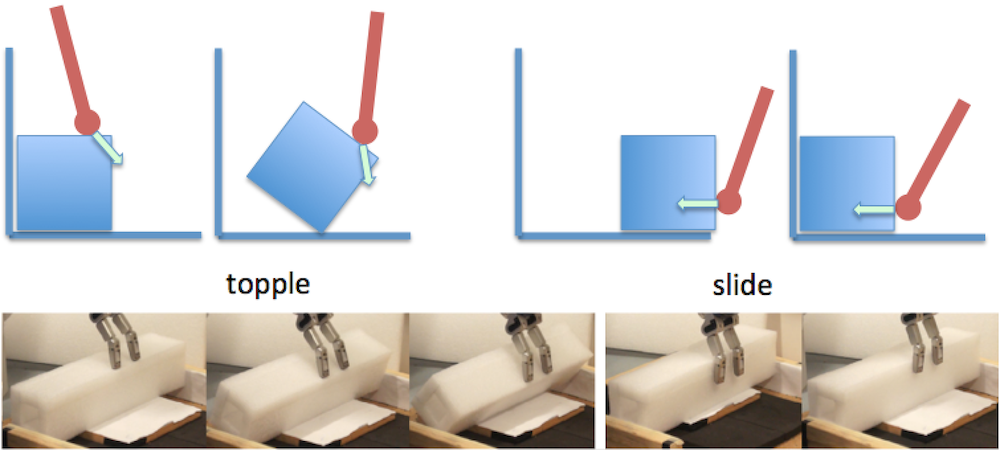
\includegraphics[width=\linewidth]{images/topple}
	\caption{The topple-and-slide task.}
	\label{fig:topple}
\end{figure}
%ENDFIGURE

\section{Setup}

\subsection{Actuation and Sensing}
\label{sec:actuation_and_sensing}

Experiments are conducted using a 7 DOF Barrett WAM robot arm with attached 4 DOF Barrett BH-280 Hand, built by Barrett Technology (MA, USA).
A 6-axis force-torque sensor is mounted to the wrist of the arm.
The robot hand is equipped with tactile arrays on the fingers and palm.
Joint torque sensors are embedded in each of the 3 fingers.
Position control of the arm occurs at 500Hz and all sensors are sampled at 125~Hz, which is reduced to 2.5~Hz during preprocessing~(see section~\ref{sec:preprocess}).

\subsection{Kinesthetic Teach and Play}
\label{sec:kinesthetic_teach_and_play}

Example trajectories are demonstrated to the robot via a kinesthetic teach-and-play interface.
The system records pose estimates of the arm at the rate of 500~Hz and the result is saved for future playback.

\subsection{Software Architecture}
\label{sec:software_architecture}

Our real-time control framework runs on top of the {\em libbarrett} real-time systems library \cite{libbarrett}, and is used during demonstration and autonomous execution.
We also use it to record and play back data streams that are time-synchronized with the motion.
See Chapter~\ref{chap4} for further details.

\subsection{Experimental Testbed}
\label{sec:testbed}

The block used for the experiment is a rectangular prism made of medium-density polyethylene foam, with length 48.5~cm, width 10.5~cm and height 10.5~cm.
Two parallel walls of length 28.5~cm and width 6.5~cm are used to prevent the block from sliding sideways out of the workspace.
The distance between the walls is 49~cm.
As shown in Figure~\ref{fig:topple}, a wall is used to limit the final sliding motion and leave the block in its original location, ready to be toppled again.
The walls are lined with paper to decrease the coefficient of friction between the block and the walls for smoother operation.


In our experiments, different environments are defined by the Cartesian product of three sets of environment property values for $P$ = \{$P_{m}$, $P_{\mu}$, $P_{c}$\}, yielding a total of $8 \times 6 \times 3 = 144$ different environments.
These values are shown in Table~\ref{table:property_set}.

\begin{table}[h]
\centering
\begin{tabular}{l|l}
$P_m$ (g)   & \begin{tabular}[c]{@{}l@{}}425, 650, 875, 1100,\\ 1325, 1550, 1775, 2000\end{tabular} \\ \hline
$P_\mu$      & \begin{tabular}[c]{@{}l@{}}0.441, 0.505, 0.616,\\ 0.768, 0.911, 1.136 \end{tabular}            \\ \hline
$P_c$ (mm/N) & 0.294, 2.484, 0.978
\end{tabular}
\caption{Mass, coefficient of Coulomb static friction and compliance property sets, as measured for a variety of blocks and surfaces.}
\label{table:property_set}
\end{table}

\subsection{The Block Topple-Slide Task}

Toppling, as defined in \cite{Lynch1999}, consists of two high-level phases: rolling and settling.
In the rolling phase, the robot pushes the block up onto a toppling edge, which is perpendicular to the robot's movement, until the center of mass of the block is directly above the edge.
During the settling phase, the block falls under gravity and lands on a new face before coming to rest.

As it is difficult to ensure the block's center of mass is above the edge following the rolling phase, the prescribed motion is developed so as to have the robot maintain contact with the block throughout the settling phase, to the extent that this is possible.

Once the block has settled, the robot then proceeds to slide the block across the surface of the table until the block has come to a stop back at its initial pose.
Figure~\ref{fig:topple} depicts the topple-slide task with a sequence of images.

\section{Procedure}

%%%%DMT%%%%
%TODO: cut down the detail! (maybe a simple graphic would suffice)
%%%%DMT%%%%

\subsection{Learn the Task Trajectory}

A human expert demonstrates the topple-slide trajectory (Figure~\ref{fig:topple}) via kinesthetic teaching.
The robot is fixed to the table so as to not introduce additional variance in the recorded data due to base motion.
The demonstrating user performs the task in about 6~s.  
The motion is then manually tuned so that the reference trajectory succeeds for the topple-slide task for a variety of combinations of block mass, coefficient of friction, and compliance (see section~\ref{sec:actuation_and_sensing}).

\subsection{Record Sensory Dataset $\mathbf{D}$}
\label{sec:preprocess}

The prescribed motion is repeated over a series of trials $h \in [1\cdots n_h]$ for each property set $p \in P$, yielding the complete raw sensory data set $D$. 
We use $n_h=20$ repeated trials.
Before training our model, we pre-process the data as follows.
The sensory data is resampled to 5~Hz after applying a 200~ms mean box filter. 

We whiten each data set to support meaningful comparisons between sensors -- by shifting data collected from each sensor to have zero mean and a variance of one -- across all trials $h \in [1 \cdots n_h]$ and property sets $p \in P$.  
In our experiments we use $n_s=110$ sensors across $n_t=18$ time samples.
This yields a complete input vector of size $n = 1980$ for each manipulation trial.

\subsection{Feature Selection}

Following the equations in section \ref{sec:feature_selection}, we compute the $\Gamma$ for each element in $\mathbf{x}$.
We select $\Gamma_{\min}$ so as to select $0.1 \times n$ features.% in order to achieve an appropriate balance between bias and variance.
%In practice, we keep only 5\% of the original sensory features while increasing the prediction accuracy as compared to the default of using the unreduced set.

\subsection{Partial Least Squares Modeling}
Following PLS, we obtain the $\mathbf{\beta}$ coefficients.
We can make the representation more compact by further choosing only the $\mathbf{\beta}$ coefficients of largest magnitude.
In practice, we are able to make a further reduction of around 40\% without any significant impact on the prediction accuracy, as shown in Figure~\ref{fig:online}.

\subsection{Online Prediction}

%Once the model has been established using the above steps, it can be run in real-time on-board the robot as it collects novel sensory stream data during the block topple-slide task.
%%%%%
%%DMT removed:
%%As one would expect, the prediction of environment properties is most accurate once the robot has accumulated sensor readings throughout the entire motion.
%%However, we are also able to make predictions in an on-demand fashion, without having to wait until the entire motion has completed.
%%%%%
We start by parsing the entire motion into a series of key time-phases, $t^*$.
We define each $t^* \in T$ as a time-phase wherein at least $K$ sensors have received a $\Gamma$ larger than a certain value.
%This ensures that we make predictions only once it actually plausible to do so.
In practice, we choose a minimum $\Gamma$ so that $K=0.1 \times n_s$.
By training separate models in this fashion, we are able to make predictions as soon as the robot enters any phase of the motion involving selected features.
Figure~\ref{fig:online} demonstrates the prediction performance on-board the robot as it executes the task.

\subsection{Calculating environment properties}
\label{sec:property_calc_}
In order for the robot to discover a mapping between sensor readings and environment properties, a unique numerical approximation of the underlying property must be calculated.
See Figure~\ref{fig:property_calc} for a graphical overview of how the coefficient of friction and compliance are calculated.

\paragraph{Mass} 
The mass of each unit is approximated using an off-the-shelf kitchen scale.

\paragraph{Friction coefficient}
We first place the foam block atop a surface lined with the frictional material we are measuring. 
We then gradually incline the surface until the block begins to slide.
We capture the inclination at the point of sliding as $\theta$.
We finally approximate the coefficient of static friction of the frictional material to be 
$$
\mu = tan~(~\theta~), 
$$
which we also assume to be a fair approximation to the coefficient of kinetic friction.

\paragraph{Compliance}
As an estimate of the compliance of each type of foam, we set a rigid solid of known mass $m$ atop a solid block of the foam we are measuring.
The dimensions of the rigid solid and the foam solid are identical.
We then measure the compressional displacement, $d$, of the top of the foam solid using standard calipers.
Finally, we approximate the compliance of the foam to be 
$$
c = d~/~(~m~\cdot~g~),
$$ 
where $g$ is acceleration due to gravity.

\begin{figure}[]
	%\centering
    \begin{subfigure}[]{0.438\linewidth}
        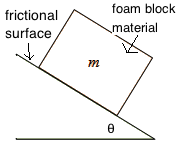
\includegraphics[width=\linewidth]{images/friction}
        \caption{Friction: ~~$\mu = tan~(~\theta~)$}
        \label{fig:friction}
    \end{subfigure}
    ~~~~
    \begin{subfigure}[]{0.490\linewidth}
        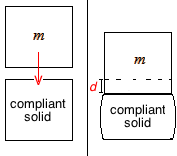
\includegraphics[width=\linewidth]{images/compliance}
        \caption{Compliance: ~~$c = d~/~(~m \cdot g~)$}
        \label{fig:compliance}
    \end{subfigure}
    \caption{Calculating numerical representations of environment properties (a) coefficient of friction, $\mu$, and (b) compliance, $c$. $\theta$ represents the inclination of the frictional surface at the precise point the foam block begins to slide. Acceleration due to gravity is represented by the constant $g$.}
    \label{fig:property_calc}
\end{figure}

%------------------------------------------------------------------------------------
\section{Results}
%%%%%DMT%%%%%
%%%DONE: video - label gaps in estimator output
%%%TODO: video - mark topple and slide phases on data output plots
%%%%%DMT%%%%%
In what follows below, we comment on topple-slide experiments carried out with the robot hand, as well as with the spherical probe.
We also encourage the reader to watch the supplemental video associated with this paper.

%%%%%%%%%%%%%%%% TVR visualization

$\Gamma$ selection helps focus attention on specific sensors and motion-phases that are particularly likely to provide information useful to predicting environment properties.
Figure~\ref{fig:tvr_tables} illustrates the selected features for the topple-slide task as executed by the robot arm with either the Hand or spherical probe as end effectors.
Notice how clusters of $\mathbf{x}^*$ can be interpreted as defining important sensory events in the task sequence, which the robot should pay most attention to.
The yellow shaded region corresponds to the topple phase and the blue shaded region corresponds to the slide phase.
The motion phases where the arm is not in contact with the object are identified as being unimportant, as are the phases that mark the beginning and end of both of the topple and sliding phases.
In terms of sensors, the joint velocities, $jv_n$, are generally unimportant, with the exception of joint 6. 
Joints 2, 4, and 6 provide task-relevant information in their sensed torques and positions.
Similar results are also obtained with the full hand attached to the robot arm, in which case there are over a hundred sensors sampled across 18 time phases of the motion.
With the hand in place, the key sensors are determined as being the task wrench $\omega$, as measured by the force-torque sensor, the fingertip torques, $f$, and the fingertip tactile readings, $a$.

%%%%%%%%%%%%%%%%%%
%%% DMT added: 
It may be noted that a simple contact/no-contact feature identifier might yield similar segmentations of the overall task in this case.
However, this would require an explicit model that extracts contact information from sensory inputs.
Our method identifies key points in the motion without any manually-tuned sensory features.
%%%         **Perhaps this is good material for related work section
%%%%%%%%%%%%%%%%%%

%%%DMT%%%%%%%%%%%%%
%%%TODO: compare TVR to simpler method e.g. contact no-contact thresholding
%%%DMT%%%%%%%%%%%%%
%\begin{figure}[tb]
%  \centering
%% 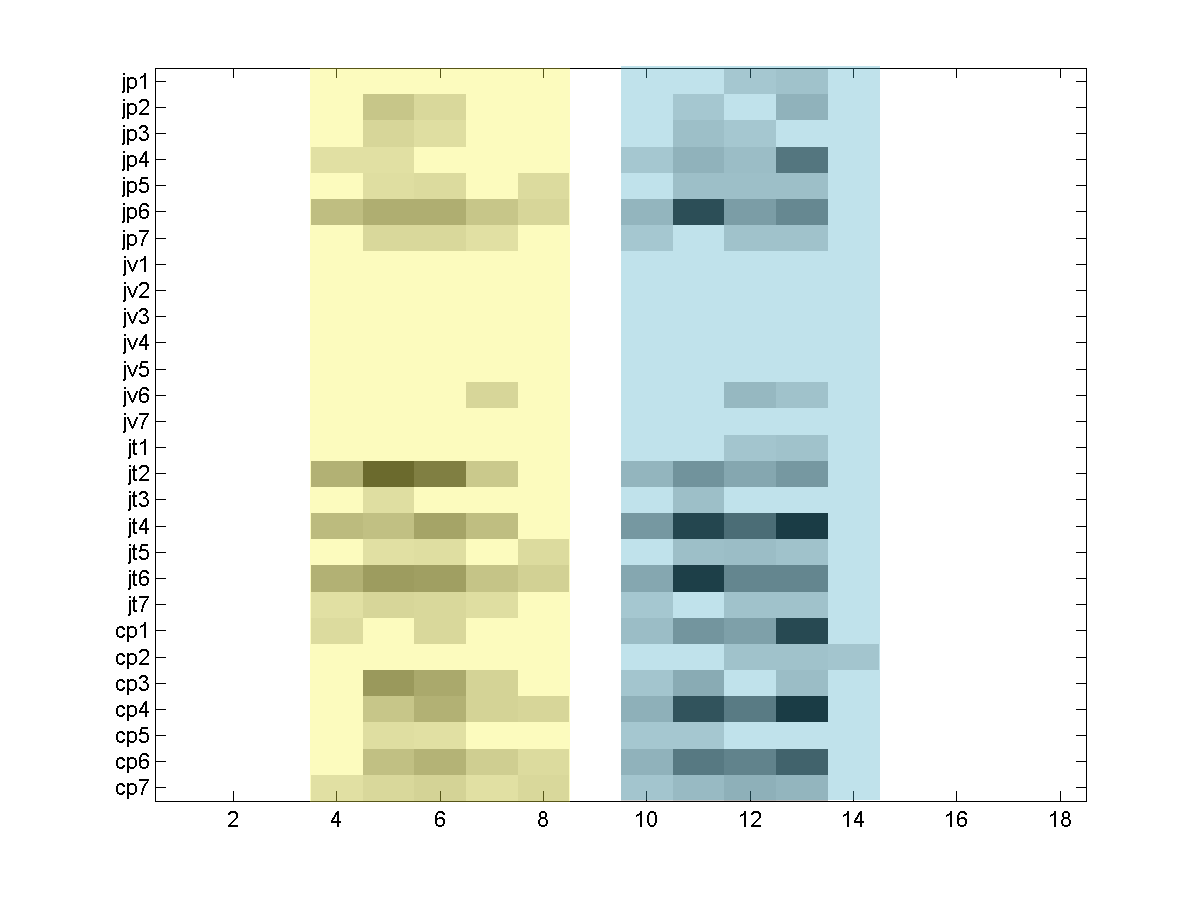
\includegraphics[width=\linewidth]{images/TVR_table}
%  \includegraphics[width=\linewidth]{images/TVR_table-probe}
%% \includegraphics[width=\linewidth]{images/TVR+photos}
%  \caption{Visualization of Task Variance Ratio ($\Gamma$) features selected for joint position (jp), velocity (jv), torque (jt), and Cartesian pose (cp) measurements. The intensity of each gray rectangular region is proportional to its $\Gamma$ value.}
%  \label{fig:TVR}
%\end{figure}


%%%%%%%%%%%%%%%%% Effect of TVR feature selection on the mass predict

%%%DMT%%%%%%%%%%%%%
%%%DONE: Error bars
%%%DONE: axis units
%%%DMT%%%%%%%%%%%%%
%\begin{figure}[tbh]
%       \centering
%%        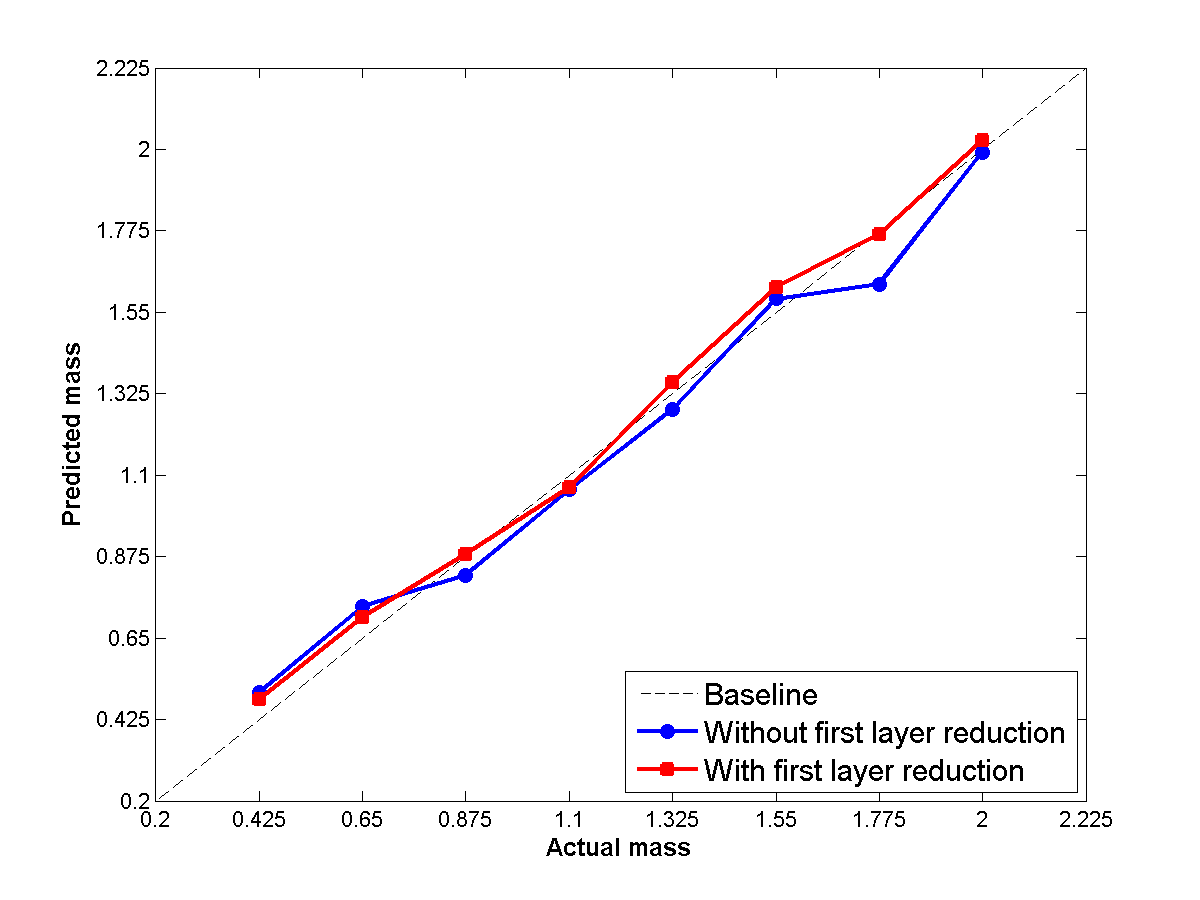
\includegraphics[width=\linewidth]{images/bomo_bomw_comp}
%       \includegraphics[width=\linewidth]{images/feature_sel_w_vs_o_bar}  %% new figure:  comparison with 10% feature selection
%       \caption{Effect of 5\% $\Gamma$ feature selection on mass predictions. Accuracy improves to within 1 measurement unit for all tests.}
%  \label{fig:TVR-perf}
%\end{figure}


To determine the impact of the $\Gamma$ feature selection, we compare mass predictions obtained using the inclusion of all features, i.e., no feature selection, and those obtained when $\Gamma$ feature selection is used to select a subset of 5\% of the the original features.
This is applied to the manipulation task as executed using the spherical probe.
In both cases, a non-reduced partial least squares model is constructed and leave-one-out-cross validation (LOOCV) test is considered for performance evaluation.
As shown in Table~\ref{fig:TVR-perf}, the result produced using the significantly reduced subset of input features is in most tests better than that obtained when using all the features.
Also, as can be seen in Table~\ref{tbl:tradeoff}, applying up to 20\% $\Gamma$ feature selection to the incoming datastreams enables real-time operation in terms of both data-transfer bandwidth and prediction runtime.
%For experiments with the robot hand, reductions of up to 90\% using $\Gamma$-based feature selection continue to yield improvements.
%This larger reduction is possible because of the large number of tactile sensors that are available with the hand.

%%%%%%%%%%%%%%%%%% Effect of Beta reduction on the mass predict

If desired, a fixed subset of the largest computed partial least squares coefficients can be used for the final prediction, instead of the full set, $\mathbf{\beta}$. 
In practice, a 40\% reduction in the number of coefficients yields only a minimal reduction in the quality of the prediction.

% Figure~\ref{fig:beta-perf} shows the effect of choosing increasingly small subsets of the coefficients. 
% 
% \begin{figure}[ht]
%   \centering
%   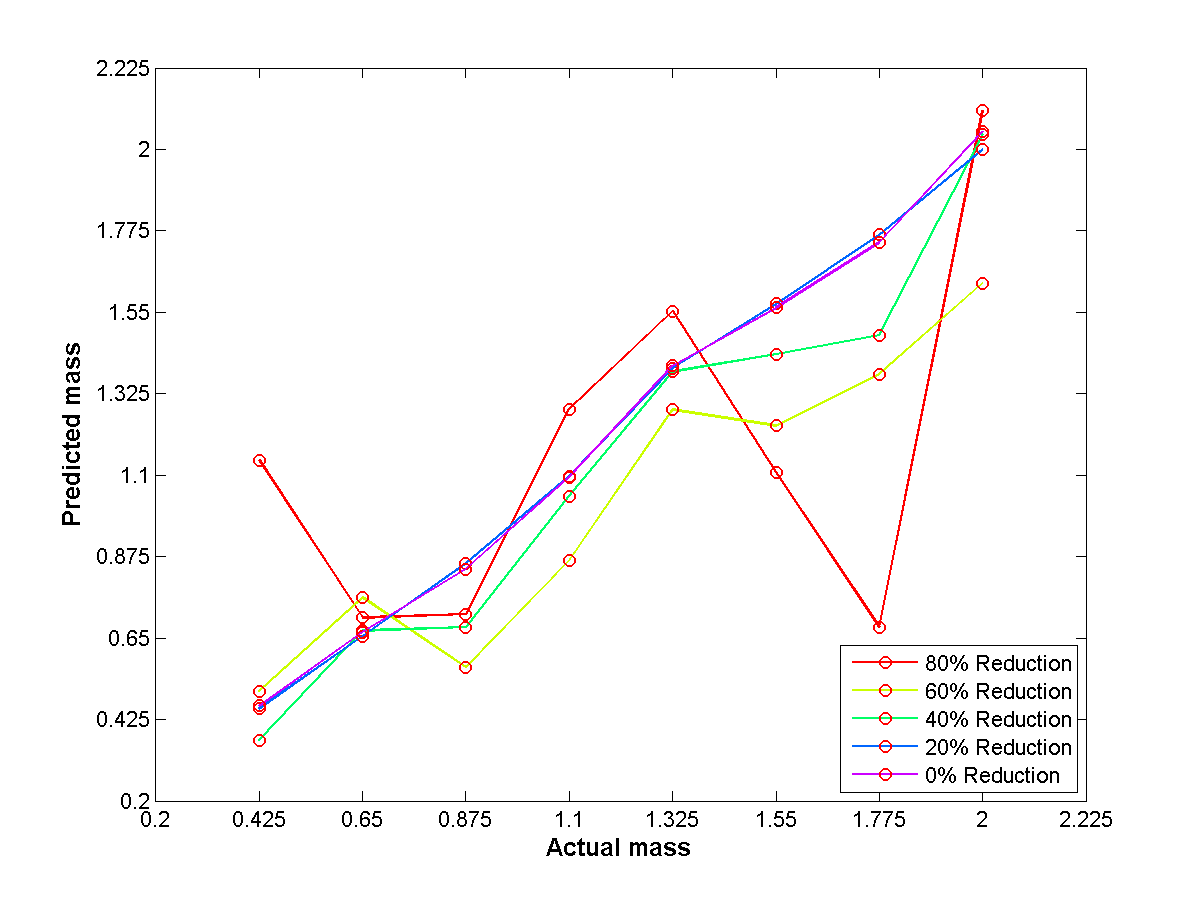
\includegraphics[width=\linewidth]{images/beta_reduc_comp}
%   \caption{Effect of partial least squares dimensionality reduction on mass prediction.}
%   \label{fig:beta-perf}
% \end{figure}

%%%%%%%%%%%%%%%%%%  Comparison to other methods

%%%DMT%%%%%%%%%%%%%
%%%DONE: Include LOOCV results in comparison (Elaborate more on generalization potential of each approach)
%%%DONE: Include mean and standard deviations for each across many runs (use dummy values for now)
%%%TODO: Replace dummy standard deviations for real ones
%%%DMT%%%%%%%%%%%%%
To validate our choice of partial least squares (PLS), we compare the results against three other methods:  principal component regression (PCR), least squares regression (LSR), and naive Bayes classification (NBC).
%In PCR, only correlations in the input space are considered when establishing a linear space for use during regression.
For LSR, we regularize the solution using ridge regression.
For NBC, a new sensory stream is treated as input to a classification problem, and the classifier is constructed using naive Bayes that assumes that all features in $\mathbf{x}$ are independent.
Using the repeated trials for the given set of environment properties, a normal distribution is constructed for each element of $\mathbf{x}$, and the likelihood of a new value of $\mathbf{x}$ belonging to the same class is simply modeled as the product of the individual element likelihoods.
The environment properties of the most likely class are then returned as the prediction.
All four methods are evaluated using LOOCV, and are applied to $\mathbf{x^*}$, i.e., after $\Gamma$ feature selection.
The results for mass prediction show that PLS yields the best predictions, with respective mean errors for PLS, PCR, and LSR and NBC of 33.3, 56.4, and 84.9, and 282.6, 
with respective standard deviations of 4.2, 8.4, 14.6 and 83.2 as measured in $grams$.

%%%%%
%%DMT removed:
%%It can be shown that PLS seeks directions of high variance \emph{and} high correlation with the response, in contrast to principal components regression, which only seeks directions of high variance.
%%%%%

%%%%%%%%%%%%%%%%%%  Online property prediction results
Figure~\ref{fig:online} illustrates online mass prediction results. The robot is able to make predictions at any key time-phase, $t^{\star}$, each characterized by a high $\Gamma$ for many sensors. This is accomplished through building multiple models, each spanning the data from the start of the motion to some $t \in t^{\star}$.
%illustrates the result for the mass predictions provided by the multiple PLS models.

These results are obtained wherein the robot trains on $m = \{425, 650, 875, 1100, 1550, 1775, 2000\}$ as measured in $g$ and is then tested using sensory data obtained for $m=1335$ g.
The result shows predictions being made using increasingly fewer selected features or reduced PLS dimensions, as noted in the caption.
Also, the predictions improve as the motion progresses and more selected features are observed.  
%%%%%%%%DMT%%%%%%%%
%TODO: all three too similar: refocus on speedup instead of prediction performance.
%%%%%%%%DMT%%%%%%%%
%\begin{figure}[tb]
%  \centering
%  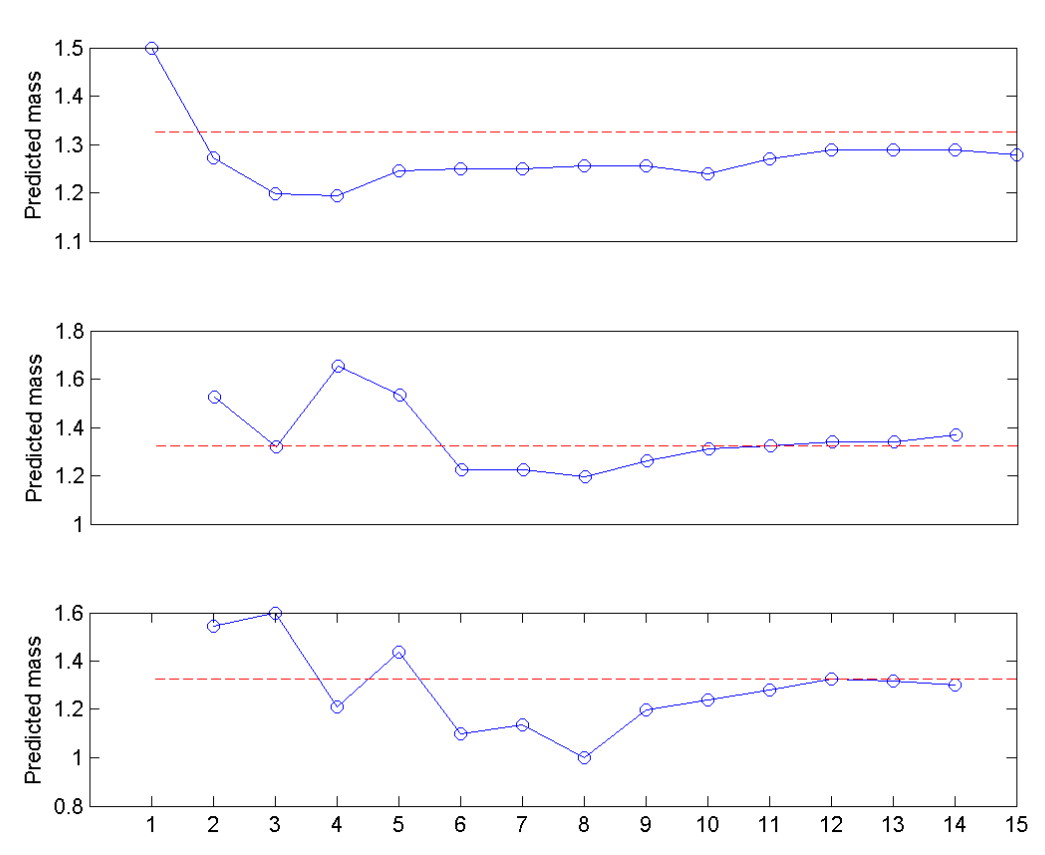
\includegraphics[width=\linewidth]{images/online_loocv_m}  %% mass predictions
%  \caption{
%    \label{fig:online}
%    Online prediction of the mass from sensory data.
%    Predictions of mass are shown at various blue points throughout the motion.
%    The dotted red horizontal line denotes the actual mass of the block.
%    The first row uses all 1650 features and no PLS reduction.
%    The second row uses a reduced set of 165 selected features without PLS reduction.
%    The third row uses 165 selected features, followed by 40\% PLS reduction.}
%\end{figure}

\begin{center}
\begin{table}[h]
\begin{tabular}{|l|l|l|l|l|l|l|}
\hline
\multicolumn{1}{|r|}{$\Gamma$ data selection:} & 5\%           & 10\%          & 20\%          & 40\%          & 70\%          & 100\%  \\ \hline
\multicolumn{1}{|r|}{\# FLOPs (approx.):}      & 32             & 65           & 131          & 263          & 461          & 659 \\ \hline
\multicolumn{1}{|r|}{Runtime (ms):}    & 0.25          & 0.5          & 1.0         & 2.1           & 3.6         & 5.1 \\ \hline
\multicolumn{1}{|r|}{Bandwidth (bit):} & 352             & 704           & 1408          & 2816          & 4928          & 7040          \\ \hline
\multicolumn{1}{|r|}{Maximum error (g):} & 69.5 & 112.7 & 96.3 & 111.4 &  107.9 & 188.3 \\ \hline
\multicolumn{1}{|r|}{\textbf{Real-time satisfied?}}        & T           & T         & T         & T/F   & F        & F        \\ \hline
\multicolumn{1}{|r|}{\textbf{Bandwidth satisfied?}}       & T           & T         & T         & F   & F        & F        \\ \hline
\multicolumn{1}{|r|}{\textbf{Accuracy satisfied?}}        & T           & T/F       & T         & T/F     & T        & F        \\ \hline
\end{tabular}
\caption{Bandwidth/runtime/accuracy tradeoff following different amounts of $\Gamma$ selection. Optimal tradeoff is achieved when between 5\% and 20\% of the data is selected using $\Gamma$. Assumes 1Mbit CANBus, 16MHz dedicated processing speed and a real-time control loop frequency of 500Hz. FLOPs are calculated using standard inner-product vector multiplication complexity of $2n-1$ for each of the three property predictions.}
\label{tbl:tradeoff}
\end{table}
\end{center}

%---------------------------------------------------------------------------------------------------------------------
\section{Discussion}

%TODO: reorganize

Our prediction framework uses unlabeled sensory data streams, collected during a manipulation task, to make reliable real-time predictions about environment properties that cannot be visually observed, i.e., mass, friction, and compliance, given the existence of relevant training examples.
Sensors or motion phases that are observed to be noisy are readily discounted by our method.
The results show that the task variance ratio, $\Gamma$, provides a simple means for feature selection, identifying important sensors and motion-phases supporting real-time predictions, and which furthermore improves the resulting partial least squares predictions.

While predicting environment properties from labeled training data could be an obvious application of linear regression, this is in practice problematic because the training data for our scenario consists of a relatively small sample size (low hundreds) embedded in a high dimensional space: $\mathbf{x}$ can contain thousands of sensory measurements.
Furthermore, the large number of measurements required to make accurate predictions prohibits real-time operation.

Although PLS utilizes a dimension reduction technique by using a few latent factors, it cannot avoid the sample size issue since a it has been proven that a reasonable sample size relative to the number of parameters is required to estimate sample covariances consistently \cite{chun2010sparse}.
Thus, PLS works best under the conditions of large sample sizes and/or small numbers of input variables. 

When combined with $\Gamma$ feature selection, our results show PLS superior to other regression algorithms which do not leverage input and output correlations in their calculations.
Unlike PCR, PLS uses $\mathbf{y}$ (in addition to $\mathbf{x}$) to construct its principal directions.
Thus, its solution path is a nonlinear function of $\mathbf{y}$ \cite{Friedman2001}.
In addition to outperforming the other benchmark prediction methods for the task, PLS also provides a further opportunity for dimensionality reduction if desired. 

Due to the model-free nature of our approach, the prediction framework works for virtually any combination of sensor modalities, including tactile-pressure, Cartesian wrench and joint-torque, 
which enables easy experimentation to determine the optimal tradeoff between sensor usage and prediction accuracy.

One limitation of our approach is that $\Gamma$ can be misleading, such as in the case of noise-free features that also exhibit significant non-linearities with respect to the properties being predicted. 
Another drawback is that the learned predictive model remains specific to the prescribed motion used for the task and the specific kinematics and dynamics of the robot and environment it trained in.
The current remedy is to incorporate further training data from which to build the model when changes to the robot or its motion take effect.
In future work, we intend to examine how the predictive model can be transferred to new settings \cite{pan2010survey}.

Our framework can also be leveraged in multiple ways in order to detect anomalous events.
Rapid changes in the predicted environment properties, such as object compliance, is a signal of an anomaly.
Also, implicit in the computation of $\mathit{Var}^{enviro}$ is a model of what value a sensory feature should have at a given point in the motion.
This allows a motion anomaly to be signaled if a number of sensors each begin to signal anomalous values at a given point in time, or a sensor anomaly to be signaled if a single sensor begins to consistently produce anomalous readings.

\begin{figure}[]
	%\centering
    \begin{tabular}{c}
        \begin{subfigure}[]{1\linewidth}
            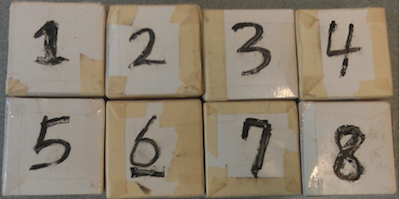
\includegraphics[width=\linewidth]{images/setup_m}
            \caption{Eight units of 0.225kg mass which are used to vary the mass of the manipulated foam block from 0.445kg to 2kg.}
        \end{subfigure} \\
        \begin{subfigure}[]{1\linewidth}
            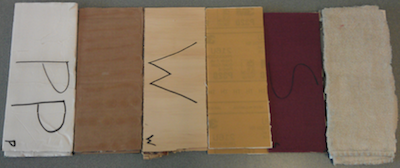
\includegraphics[width=\linewidth]{images/setup_f}
            \caption{Six surface frictions (from left to right): paper, plastic, wood, fine-sandpaper, coarse-sandpaper, cloth.}
        \end{subfigure} \\
        \begin{subfigure}[]{1\linewidth}
            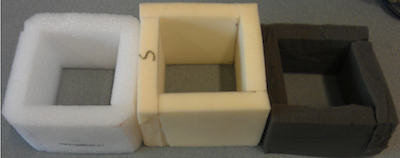
\includegraphics[width=\linewidth]{images/setup_c}
            \caption{Three levels of compliance (from left to right): ethafoam, seafoam, greyfoam.}
        \end{subfigure}
    \end{tabular}
    \caption{environment properties used in experiments.}.
    \label{fig:vis_properties}
\end{figure}


\begin{figure}[]
	%\centering
    \begin{subfigure}[]{0.438\linewidth}
        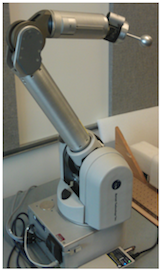
\includegraphics[width=\linewidth]{images/wam_p}
        \caption{}
    \end{subfigure}
    \begin{subfigure}[]{0.490\linewidth}
        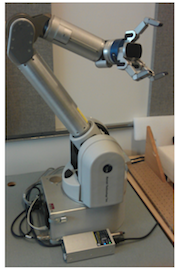
\includegraphics[width=\linewidth]{images/wam_h}
        \caption{}
    \end{subfigure}
    \label{fig:wam}
    \caption{We performed two experiments using the WAM robot with (a) spherical probe and (b) BarrettHand as end-effectors.}
\end{figure}


%FIGURE 
%\begin{figure}[]
%	%\centering
%    \begin{center}
%	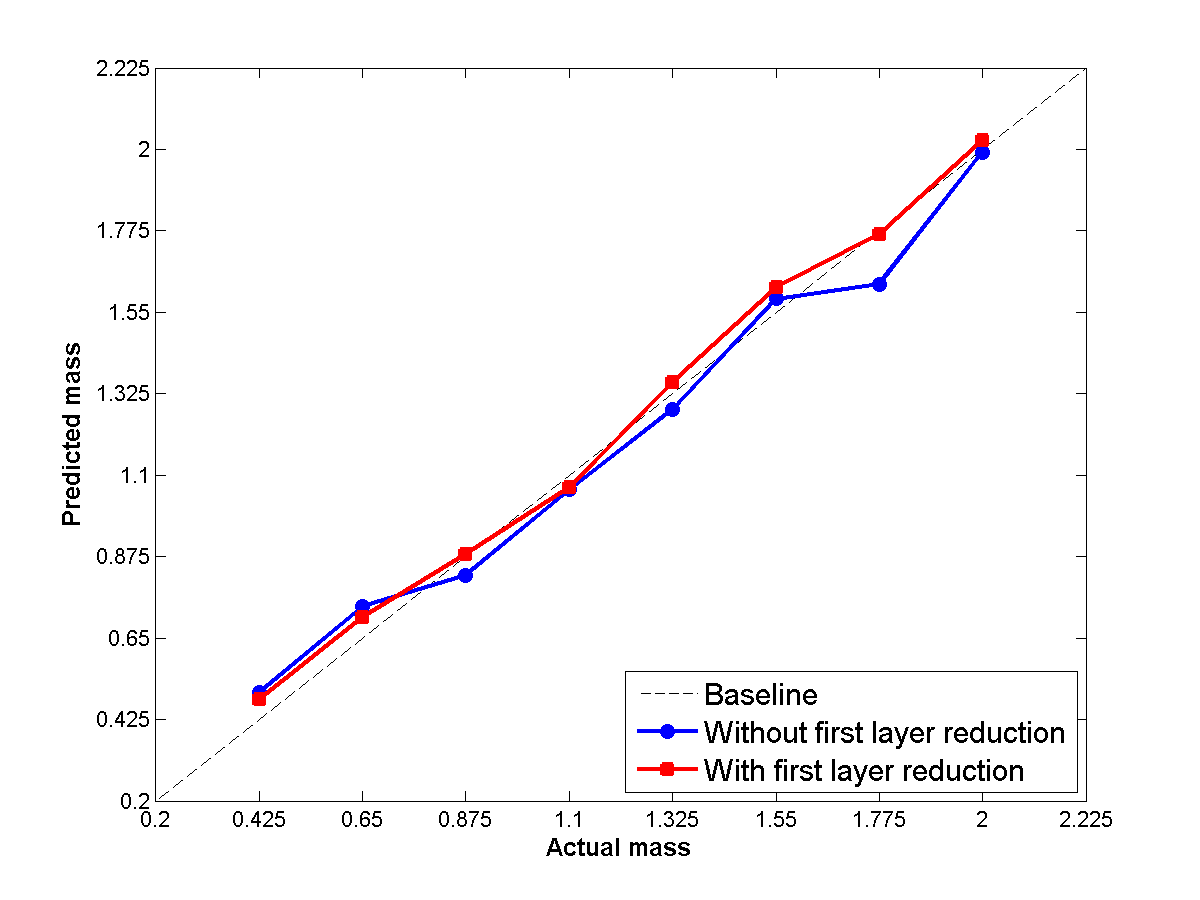
\includegraphics[width=\linewidth]{images/tvr_reduc}
%    \end{center}
%	\caption{Prediction performance of the learning system both with and without task variance ratio feature selection. Follwoing feature selection, we achieve improved performance while ignoring 75\% of the input data.}
%	\label{fig:tvr_reduc}
%\end{figure}
%%ENDFIGURE

\begin{table}[h]
\centering
\begin{tabular}{c|c|c|}
\cline{2-3}
\multicolumn{1}{l|}{}                  & \multicolumn{2}{c|}{Prediction RMSE (g)} \\ \hline
\multicolumn{1}{|c|}{Mass (g)} & PLS + $\Gamma$    & PLS Only   \\ \hline
\multicolumn{1}{|c|}{~425}           & 2.40              & 75.7         \\
\multicolumn{1}{|c|}{~650}           & 13.9              & 86.9         \\
\multicolumn{1}{|c|}{~875}           & 1.40              & 51.1         \\
\multicolumn{1}{|c|}{1100}           & 15.8              & 40.8         \\
\multicolumn{1}{|c|}{1325}           & 7.20              & 43.1         \\
\multicolumn{1}{|c|}{1550}           & 0.20              & 37.2         \\
\multicolumn{1}{|c|}{1775}           & 9.00              & 147         \\
\multicolumn{1}{|c|}{2000}           & 11.0              & 7.20         \\ \hline
\end{tabular}
\caption{Effect of 5\% $\Gamma$ feature selection on LOOCV block mass prediction root mean squared error (RMSE). Accuracy improves to within 1 measurement unit ($\pm$ 112.5 g) for all tests. Similar results are obtained for surface friction and block compliance predictions.}
\label{fig:TVR-perf}
\end{table}


%FIGURE 
\begin{figure}[]
	%\centering
    \begin{center}
    \begin{tabular}{c}
        \begin{subfigure}[]{0.8\linewidth}
            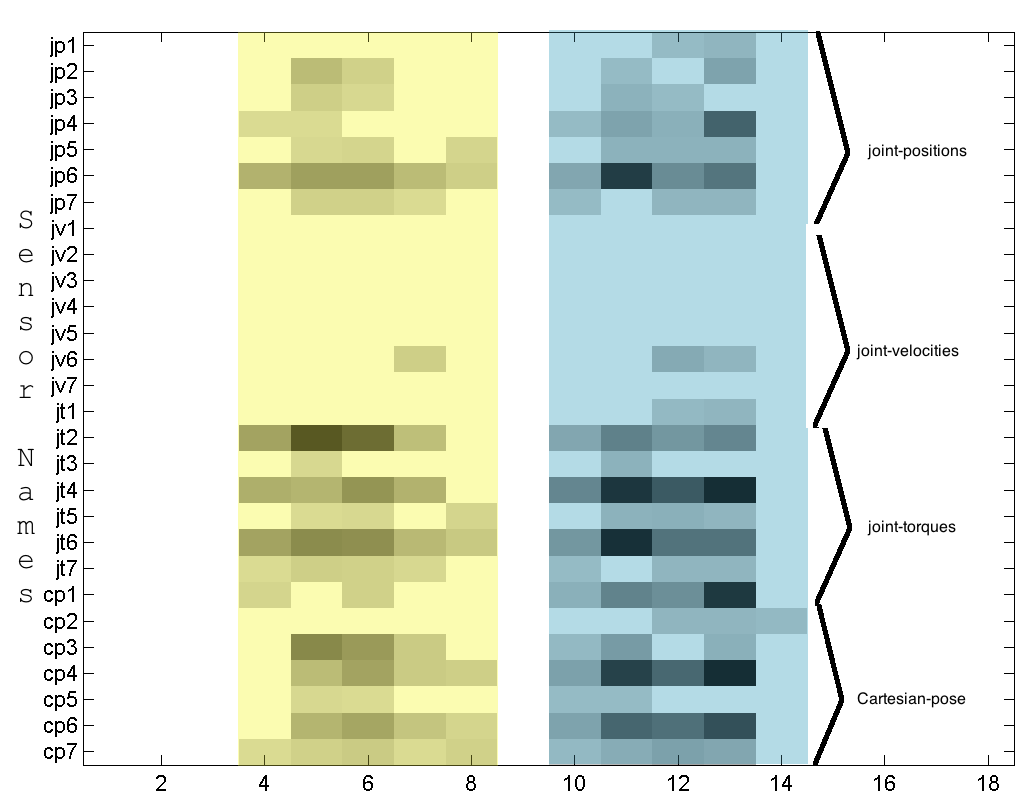
\includegraphics[width=\linewidth]{images/tvr_table_p}
            \caption{Joint-velocities are not selected due to high noise.}
            \label{fig:tvr_table_p}
        \end{subfigure}\\
        \begin{subfigure}[]{0.78\linewidth}
            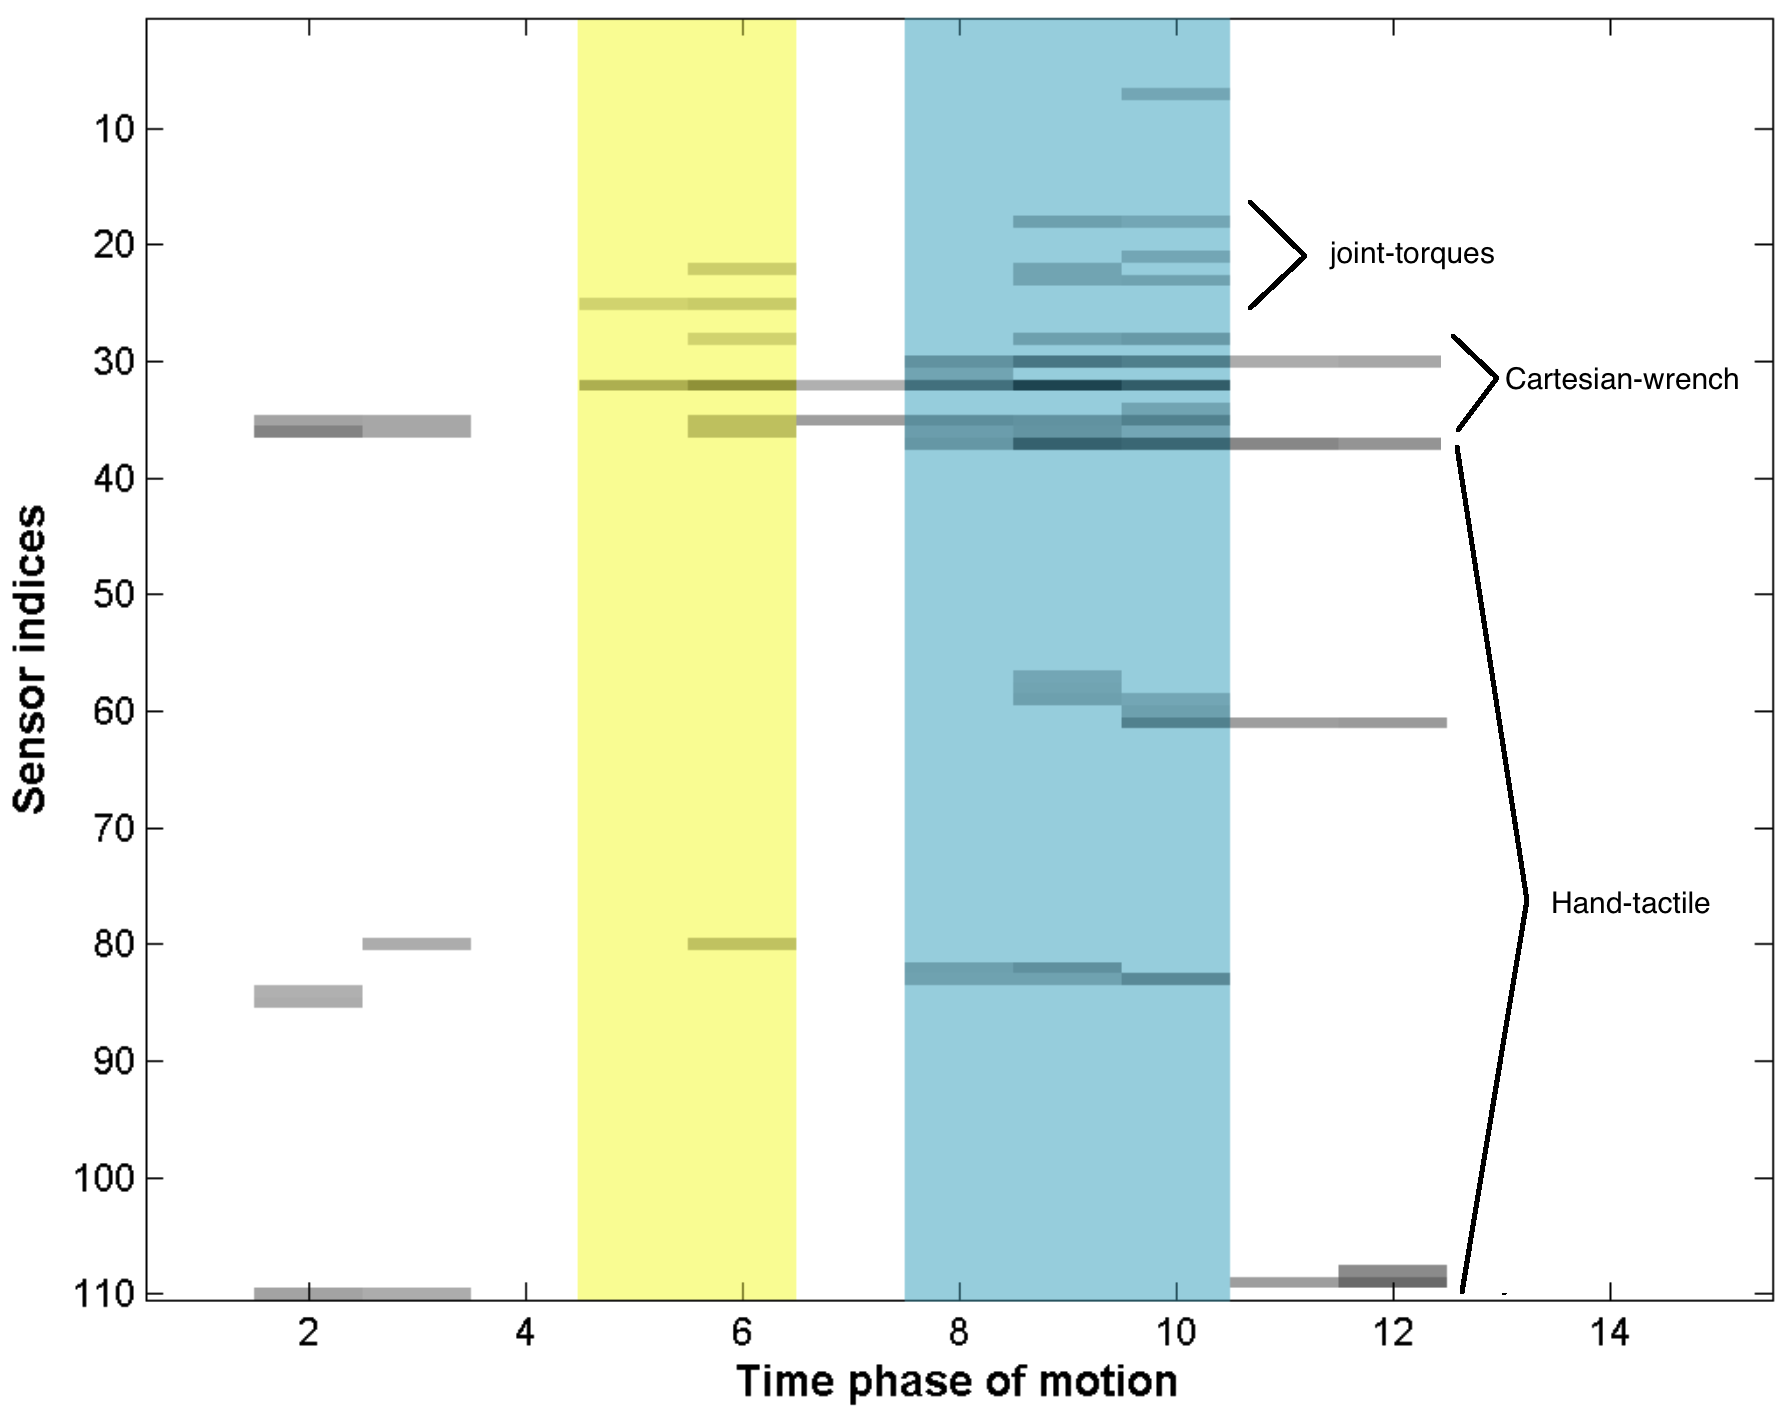
\includegraphics[width=\linewidth]{images/tvr_table_h}
            \caption{Joint-torques, Cartesian-wrench and Hand-tactile selected for providing most task-relevant information to the system.}
            \label{fig:tvr_table_h}
        \end{subfigure}
    \end{tabular}
    \end{center}
    \caption{Visualization of features selected according to the task variance ratio, $\Gamma$, of data collected using (a) robot with spherical probe and (b) robot with BarrettHand. Colour is added to signify task-phases. Gaps between task-phases signify an absence of task-relevant information within corresponding time-phases.}
    \label{fig:tvr_tables}
\end{figure}
%ENDFIGURE

%FIGURE 
\begin{figure}[]
	\centering
	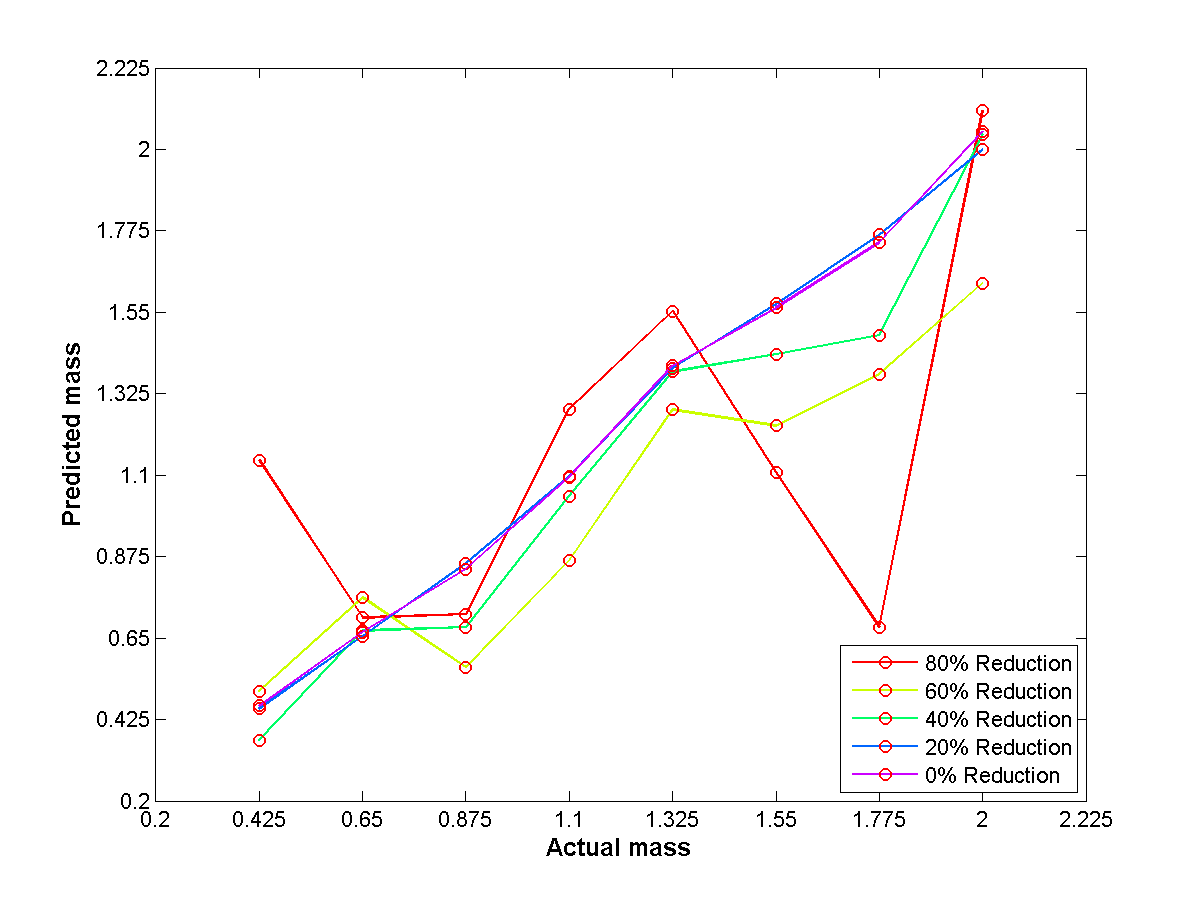
\includegraphics[width=\linewidth]{images/beta_reduc_comp}
	\caption{Effect of varying degrees of PLS dimensionality reduction on mass estimation performance. A 20\% reduction is achievable with trivial loss in estimation quality.}
	\label{fig:beta_reduc_comp}
\end{figure}
%ENDFIGURE

%FIGURE 
\begin{figure}[]
	\centering
	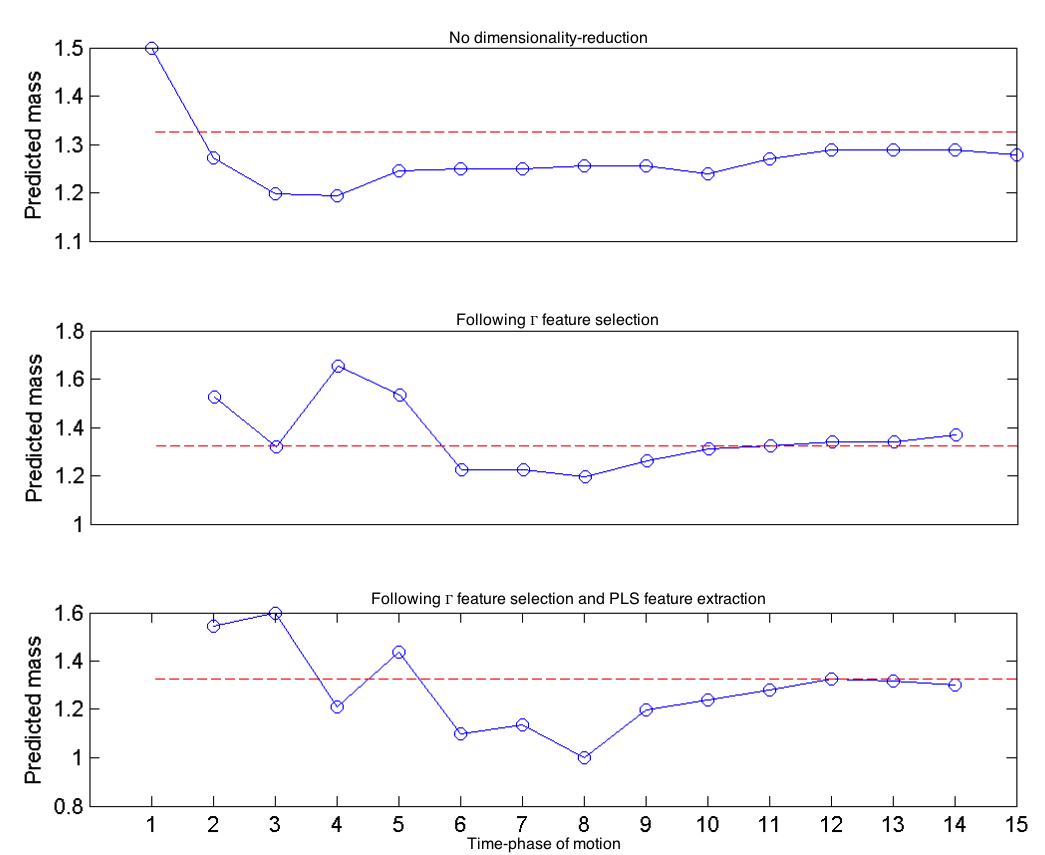
\includegraphics[width=\linewidth]{images/online_m}
	\caption{Online estimation of the mass from sensory data using varying degrees of dimensionality reduction. 
    The estimated mass of the block are shown at various blue points throughout the motion. 
    And the dotted red horizontal line denotes the actual mass of the block. The first row uses all features and no PLS reduction. 
    The second row uses a reduced set of 5\% selected features without PLS reduction. 
    The third row uses 5\% selected features, followed by 40\% PLS reduction.
    Following feature extraction step, the first and last time-phase of the motion are deemed irrelevant to the estimation task.}
	\label{fig:online}
\end{figure}
%ENDFIGURE

%FIGURE 
\begin{figure}[]
	\centering
	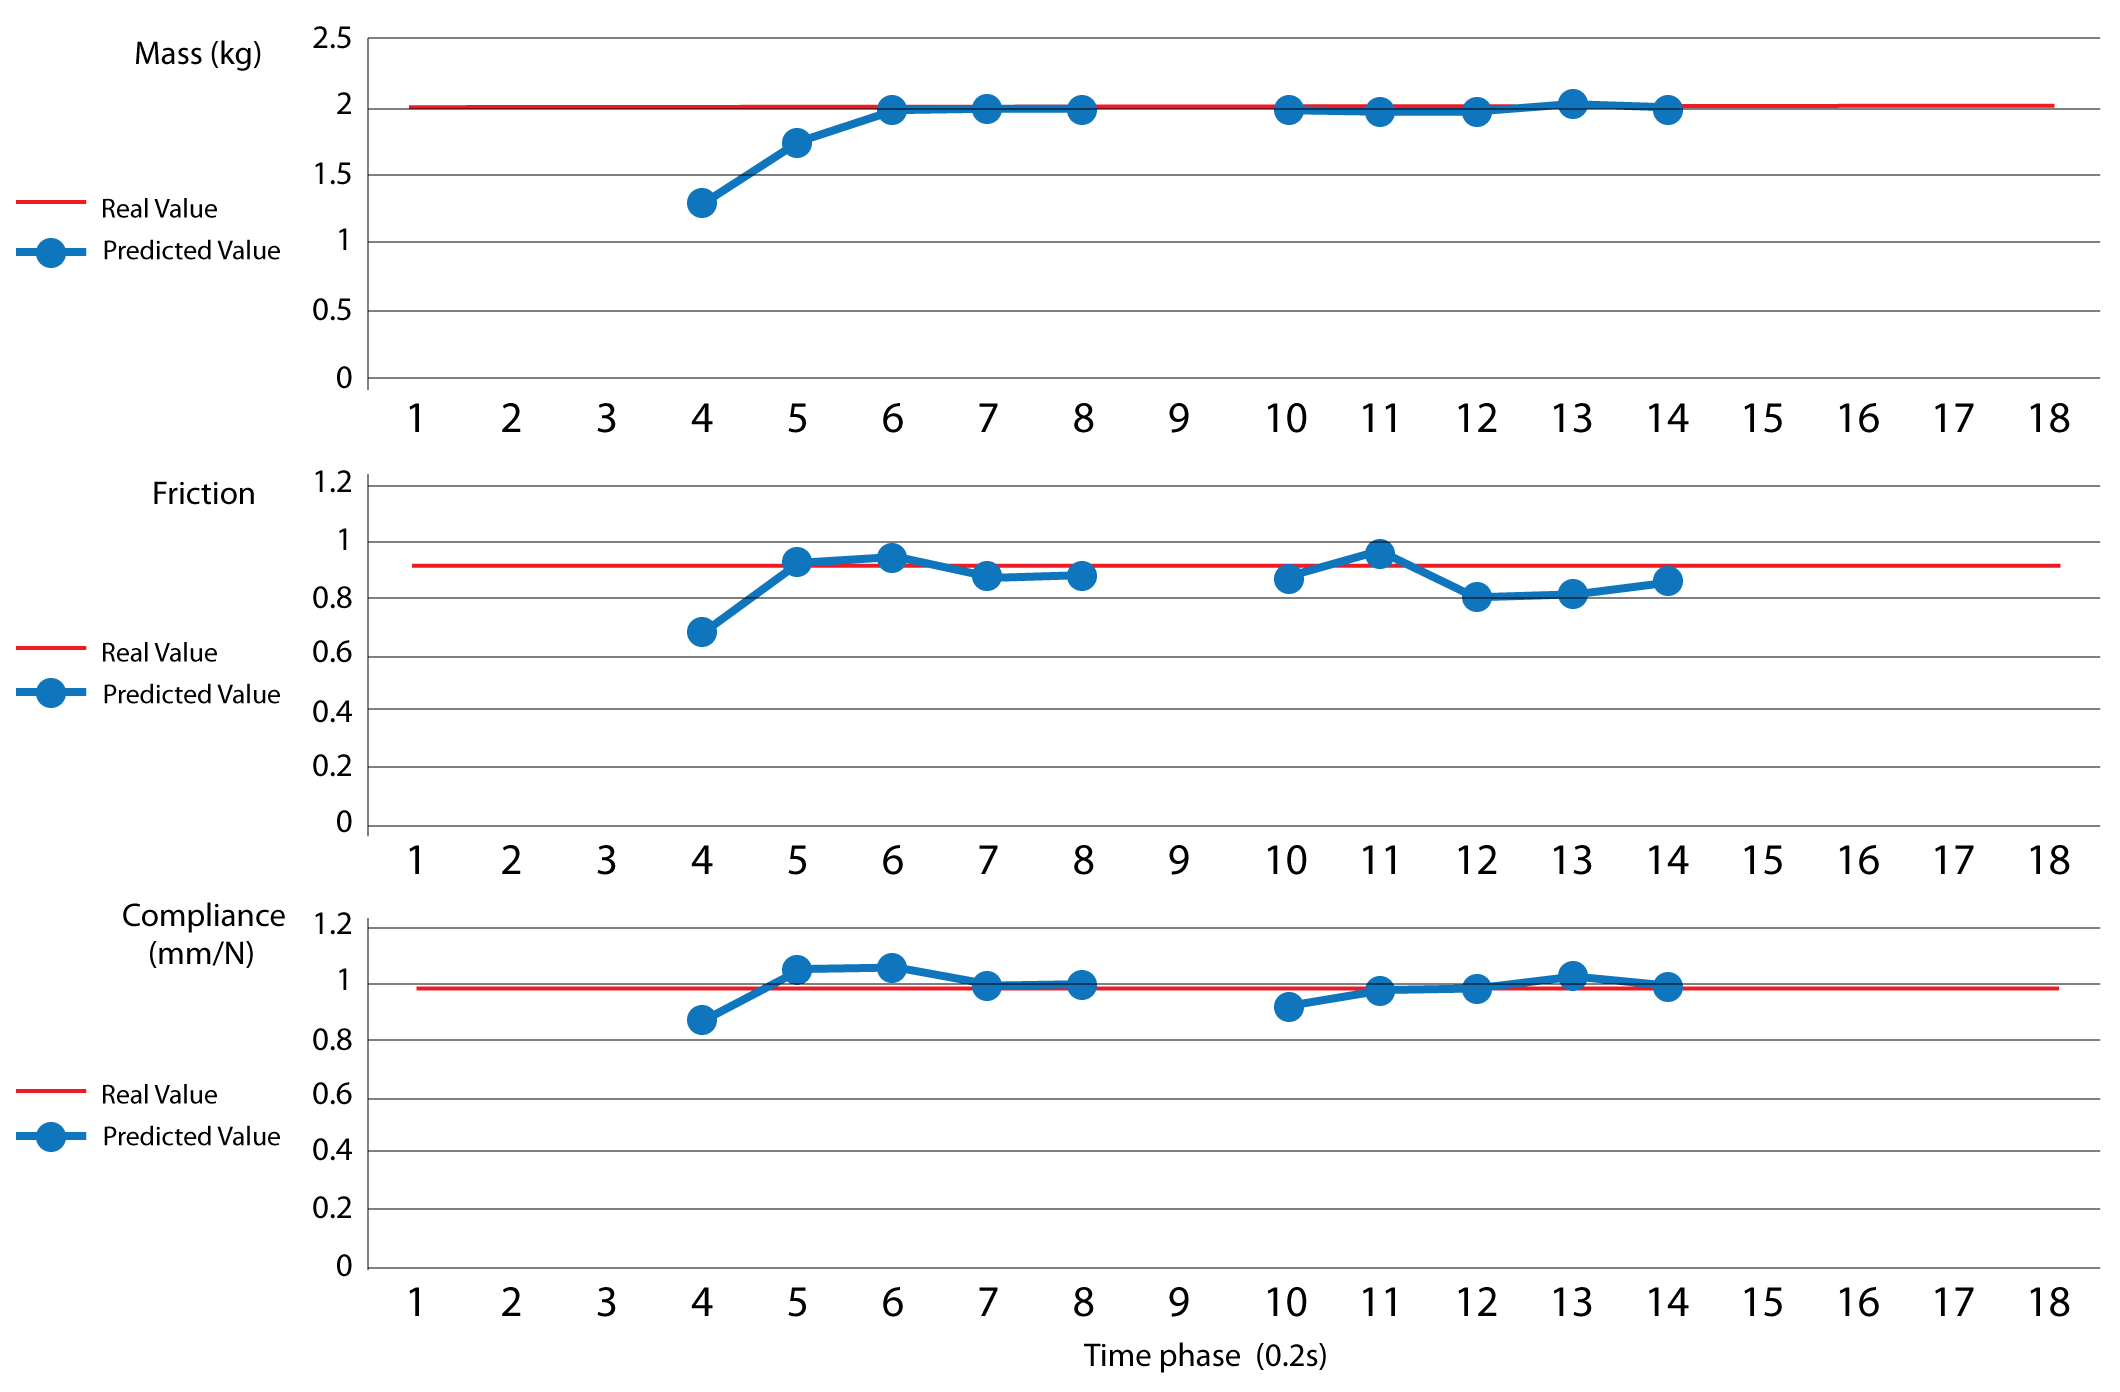
\includegraphics[width=\linewidth]{images/online_mfc_vid}
	\caption{Online estimation of mass, friction and compliance from sensory data following $\Gamma$ feature selection and PLS feature extraction. 
    Time-phases 1 through 3, 9 and 15 through 18 are ignored since sensor readings during these time-phases do not provide any information with respect to distinguishing environment properties.}
	\label{fig:online_mfc_vid}
\end{figure}
%ENDFIGURE


%%%%%%%%%%%%%%%%%%%%%%%%%%%
